\documentclass{article}
\author{Alex Hiller (11850637)}
\title{Linear Deformation of Images}
% Type-setting
\setlength{\parindent}{0cm}
\setlength{\parskip}{0.125cm}
\pagenumbering{gobble}
\usepackage[margin=2.5cm]{geometry} % Formatting
\usepackage{amsmath}      % Mathematics
\usepackage{amssymb}      % Mathematics
\usepackage{listings}     % Listings
\usepackage{esint}        % Mathematics
\usepackage{color}        % Listings
\usepackage{courier}      % Listings
\usepackage{circuitikz}   % Circuits
\usepackage{titlesec}     % Section Formatting
\usepackage{stmaryrd}     % \mapsfrom arrow.
\usepackage{svg}
\setsvg{inkscape=inkscape -z -D}
\input{/home/polluticorn/GitHub/texTemplates/texMacros}
% Section formatting
\titleformat{\section}{\huge \bfseries}{}{0em}{}[]
\titleformat{\subsection}{\Large \bfseries}{}{0em}{}
\titleformat{\subsubsection}{\bfseries}{}{0em}{}

%%%%%%%%%%%%%%%%%%%%%%%%%%%%%%%%%%%%%%%%%%%%%%%%%%%%%%%%%%%%%%%%%%%%%%%%%%%%%%%%

\begin{document}
\maketitle
\vspace{20mm}
\begin{center} {Linear Algebra (37233)\\ Written Assignment\\ Autumn 2019} \end{center}
\clearpage

The transformation of images is an image processing technique embedded in the
foundations of linear algebra. It forms the bedrock of image editing on
computers and mobiles by taking the pixels of one image and mapping their
pixels to new coordinates on a new image.

Examples of this are shrinking, reflection, dilating, stretching, displacing and
shearing. Any of these may also be done in succession.

To imagine how this is done, we must first lay some mental ideas of how we will
treat pictures.

\subsubsection{Mental Model} 

It is pertinent to recall that pictures consist of small squares
called pixels. These elementary units are uniformly coloured and each makes
up a very small part of the image. 

For example, a common image size used is $ 1920 \times 1080 $ which is a 
shorthand for saying 2073600 individual pixels. In an image of this size we have
one pixel making up less than two-millionths of the whole.

A digital image is in fact a grid of squares (Figure \ref{grid}), each with 
a single 
colour, where that colour is encoded by a number (or array of numbers in 
the case of colour images) then ordered in a 2D coordinate system (Figure
\ref{pixels}).

\subsubsection{Simplifying Assumptions} 

We will limit this small analysis to black and white pictures, as colour pictures
begin to provide the complexities of 3D arrays that are not relevant to an 
introductory survey of linear transformations of images.

Furthermore, when we examine the transformations more closely it will be assumed
that all images lay in a plane with their lower left corner at the origin, as 
depicted below:

\begin{figure}[!htbp]
    \centering
    \includesvg[width=0.4\textwidth]{normal} % No file extension.
    \caption{Reference image that will be used for transformations.}
\end{figure}


A black-and-white picture is also two-dimensional, meaning that we can organise its 
pixels in an identical fashion to how a matrix is organised.

\begin{figure}[!htbp]
    \centering
    \includesvg[width=0.3\textwidth]{grid} % No file extension.
    \caption{An example of how an image may be laid out in a matrix style
    fashion. Circles here would represent values ranging from 0 (black) to 255
    (white).}
    \label{grid}
\end{figure}

\begin{figure}[!htbp]
    \centering
    \includesvg[width=0.4\textwidth]{pixels} % No file extension.
    \caption{A closer look at how the coordinate system works for the pixels of
    an image.}
    \label{pixels}
\end{figure}

In Figure \ref{pixels}, pixels have been labelled with $ (x_n, y_n)  $ indicating
their coordinates. The $ x $-axis indicating columns and the $ y $-axis the
rows. This is pixel-by-pixel method of transforming images is integral to the
examined method in Equation \ref{svg}.


\begin{equation}
    \begin{bmatrix}
        a & b & c \\
		d & e & f \\
		0 & 0 & 1 \\	
    \end{bmatrix}
    \begin{bmatrix}
        x_n  \\
		y_n  \\
		1 \\		
    \end{bmatrix}
    =
    \begin{bmatrix}
        ax_n  + by_n + c \\
		dx_n + ey_n  + f \\
		1 \\		    
    \end{bmatrix}
    \label{svg}
\end{equation}


We can condense Equation \ref{svg} further to: 
\[%
    \mathbf{A} \mathbf{x} = \mathbf{x}'
\]%

Where $ \mathbf{A} $ is the linear transformation matrix, $ \mathbf{x} $ is our
current pixel coordinate and $ \mathbf{x}' $ is the new coordinate of our pixel.



Let us more closely examine $ \mathbf{A} $.

\[%
    \begin{bmatrix}
        a & b & c \\
		d & e & f \\
		0 & 0 & 1 \\	
    \end{bmatrix}
\]%

$ a,\ b, \ c, \ d, \ e \text{ and }f$ all correspond to different parameters that
affect the image.  The variables $ a \text{ and } e $ are used to scale, magnify 
or invert. The coefficients $ b $ and  $ d $ are to distort/warp, where as $ c $ and 
$ f $ are to displace the whole image around the coordinate system.

Let's have a closer look at how this matrix can be used to alter images.

\clearpage
\subsection{Dilation/Magnification} 

Setting $ a $ and $ e $ equal to a constant ($ \delta $) allows us to stretch the image.

\[%
    \begin{bmatrix} 
        \delta & 0 & 0 \\
		0 & \delta & 0 \\
		0 & 0 & 1 \\		
    \end{bmatrix}
    \begin{bmatrix}
        x \\
        y \\
		1 \\		
    \end{bmatrix}
    =
    \begin{bmatrix} \delta \cdot x \\ \delta \cdot y \\ 1 \end{bmatrix}
\]%

\begin{figure}[!htbp]
    \centering
    \includesvg[width=0.3\textwidth]{dilation} % No file extension.
\end{figure}


\subsection{Reflection} 
If we then set $ a $ to $-1$ and $ e $ to 1, it will reflect the image over 
the x-axis. The conjugate operations would cause a reflection over the y-axis.

\[%
    \begin{bmatrix} 
        -1 & 0 & 0 \\
		0 & 1 & 0 \\
		0 & 0 & 1 \\		
    \end{bmatrix}
    \begin{bmatrix}
        x \\
        y \\
		1 \\		
    \end{bmatrix}
    =
    \begin{bmatrix} - x \\  y \\ 1 \end{bmatrix}
    \quad
    \text{or}
    \quad
    \begin{bmatrix} 
        1 & 0 & 0 \\
		0 & -1 & 0 \\
		0 & 0 & 1 \\		
    \end{bmatrix}
    \begin{bmatrix}
        x \\
        y \\
		1 \\		
    \end{bmatrix}
    =
    \begin{bmatrix} x \\ -y \\ 1 \end{bmatrix}
\]%

\begin{figure}[!htbp]
    \centering
    \includesvg[width=0.3\textwidth]{reflection} % No file extension.
\end{figure}


\clearpage
\subsection{Shrinking/Compression} 

In a similar manner to dilation we can produce a shrinking effect if we make the
coefficient smaller than one.

\[%
    \begin{bmatrix} \vspace{1mm}
        \ 1/f  & 0 & 0 \\ \vspace{1mm} 
        0 & 1/f  & 0 \vspace{1mm}  \ \\ 
	    \ 0 & 0 & 1 \\		     
    \end{bmatrix}
    \begin{bmatrix} x\\y\\1 \end{bmatrix}
    =
    \begin{bmatrix}
        {x}/{f}  \\
        {y}/{f}  \\
		1 \\		
    \end{bmatrix}
\]%

\begin{figure}[!htbp]
    \centering
    \includesvg[width=0.3\textwidth]{shrinking} % No file extension.
    % \caption{}
\end{figure}


\subsection{Stretching} 

If we take our dilation and apply it only to one coordinate, we can stretch just
one dimension of our object.

\[%
       \begin{bmatrix} 
        \sigma & 0 & 0 \\
		0 & 1 & 0 \\
		0 & 0 & 1 \\		
    \end{bmatrix}
    \begin{bmatrix}
        x \\
        y \\
		1 \\		
    \end{bmatrix}
    =
    \begin{bmatrix} \sigma x \\  y \\ 1 \end{bmatrix}
    \quad
    \text{or}
    \quad
    \begin{bmatrix} 
        1 & 0 & 0 \\
		0 & \sigma & 0 \\
		0 & 0 & 1 \\		
    \end{bmatrix}
    \begin{bmatrix}
        x \\
        y \\
		1 \\		
    \end{bmatrix}
    =
    \begin{bmatrix} x \\ \sigma y \\ 1 \end{bmatrix}\]%

\begin{figure}[!htbp]
    \centering
    \includesvg[width=0.37\textwidth]{stretching_x} % No file extension.
    \includesvg[width=0.3\textwidth]{stretching_y} % No file extension.
    % \caption{}
\end{figure}

\begin{figure}[!htbp]
    \centering
    % \caption{}
\end{figure}


\clearpage
\subsection{Shearing/Warping} 
We're yet to use our coefficients $ b $ and $ d $, which is because they begin
to create distortions of our images which are less intuitive.

\[%
    \begin{bmatrix} 
        1 & \gamma & 0 \\
		0 & 1 & 0 \\
		0 & 0 & 1 \\		
    \end{bmatrix}
    \begin{bmatrix}
        x \\
        y \\
		1 \\		
    \end{bmatrix}
    =
    \begin{bmatrix}
        x + \gamma y \\
        y \\
		1 \\		
    \end{bmatrix}
    \quad
    \text{ or }
    \quad
    \begin{bmatrix} 
        1 & 0 & 0 \\
		\gamma & 1 & 0 \\
		0 & 0 & 1 \\		
    \end{bmatrix}
    \begin{bmatrix}
        x \\
        y \\
		1 \\		
    \end{bmatrix}
    =
    \begin{bmatrix}
        x \\
        y + \gamma x \\
		1 \\		
    \end{bmatrix}
\]%

\begin{figure}[!htbp]
    \centering
    \includesvg[width=0.3\textwidth]{shearing_x} % No file extension.
    \includesvg[width=0.3\textwidth]{shearing_y} % No file extension.
\end{figure}

\subsection{Translation} 

The image can also be moved around the plane/canvas with the $ c $ and $ f $
coefficients.

\[%
    \begin{bmatrix} 
        1 & 0 & \Delta {x} \\
		0 & 1 & 0 \\
		0 & 0 & 1 \\		
    \end{bmatrix}
    \begin{bmatrix}
        x \\
        y \\
		1 \\		
    \end{bmatrix}
    =
    \begin{bmatrix} x + \Delta {x} \\  y \\ 1 \end{bmatrix}
    \quad
    \text{or}
    \quad
    \begin{bmatrix} 
        1 & 0 & 0 \\
		0 & 1 & \Delta {y} \\
		0 & 0 & 1 \\		
    \end{bmatrix}
    \begin{bmatrix}
        x \\
        y \\
		1 \\		
    \end{bmatrix}
    =
    \begin{bmatrix} x \\ y + \Delta {y} \\ 1 \end{bmatrix}
\]%

\begin{figure}[!htbp]
    \centering
    \includesvg[width=0.3\textwidth]{translation} % No file extension.
    % \caption{}
\end{figure}

\clearpage
\section{Impact} 

The matrix format listed in Eq. \ref{svg} is that specified by the CSS standard
for the manipulation of scaleable vector graphics (SVG) files on the web.
Linear transformations like these are the core of programs like
\textit{Inkscape} (Inkscape Project 2019), which aims to allow people to 
create illustrations for free. \textit{Inkscape} in fact has a transformation
tool that uses the coefficients discussed earlier to transform digital vector objects.

\begin{figure}[!htbp]
    \centering
    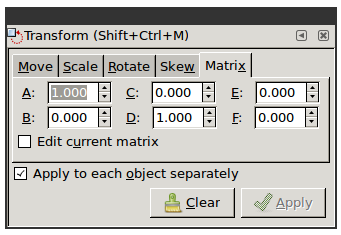
\includegraphics[width=0.3\textwidth]{inkscape}
    \caption{The \textit{Inkscape} matrix transformation tool.}
\end{figure}
    
There are an exhaustive number of libraries that list the utilise matrices as a
method for facilitating abstraction for image processing, one being PIL (now
forked to Pillow) in the Python language (Zenodo 2019). This software library
also facilitates these transformations, though not in as mathematical terminology 
as \textit{Inkscape}. The framework for image editing is so ubiquitous that it 
has made its way into W3C's standards for HTML and CSS (W3C 2019) (Mozilla
2019). 

\clearpage
\section{References} 


Mozilla, SVG Transformation, viewed 13th May 2019,

\qquad $<$developer.mozilla.org/en-US/docs/Web/SVG/Attribute/transform$>$


\vspace{2mm}
W3C, HTML and CSS, viewed 13th May 2019,

\qquad $<$www.w3.org/standards/webdesign/htmlcss$>$


\vspace{2mm}
Inkscape Project, Inkscape 0.91, viewed 13th May 2019,

\qquad $<$inkscape.org/about/$>$


\vspace{2mm}
Zenodo, Pillow, Version 3.1.0, viewed 13th May 2019,

\qquad $<$pillow.readthedocs.io/en/stable/reference/PixelAccess.html$>$



\end{document}



